\documentclass{article}
\usepackage{tikz}

\begin{document}

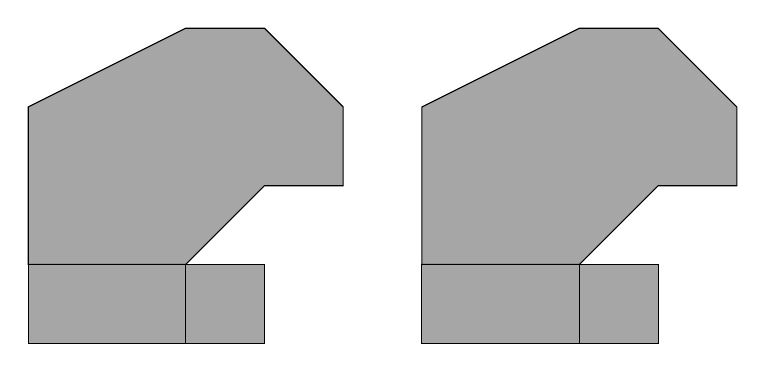
\begin{tikzpicture}[scale=0.5]
    % Left book
    \draw[fill=gray!70] (0,0) -- (4,0) -- (6,2) -- (8,2) -- (8,4) -- (6,6) -- (4,6) -- (0,4) -- cycle;
    \draw[fill=gray!70] (0,0) -- (4,0) -- (4,-2) -- (0,-2) -- cycle;
    \draw[fill=gray!70] (4,0) -- (4,-2) -- (6,-2) -- (6,0) -- cycle;
    
    % Right book
    \draw[fill=gray!70] (10,0) -- (14,0) -- (16,2) -- (18,2) -- (18,4) -- (16,6) -- (14,6) -- (10,4) -- cycle;
    \draw[fill=gray!70] (10,0) -- (14,0) -- (14,-2) -- (10,-2) -- cycle;
    \draw[fill=gray!70] (14,0) -- (14,-2) -- (16,-2) -- (16,0) -- cycle;
\end{tikzpicture}

\end{document}